\documentclass[10pt,twocolumn]{article}

\usepackage[margin=0.68in,columnsep=0.24in]{geometry}
\usepackage{amsmath,amssymb}
\usepackage{booktabs}
\usepackage{graphicx}
\usepackage{microtype}
\usepackage[dvipsnames]{xcolor}
\usepackage{hyperref}
\usepackage{titlesec}
\usepackage{caption}
\usepackage{enumitem}

\hypersetup{
  colorlinks=true,
  linkcolor=MidnightBlue,
  citecolor=MidnightBlue,
  urlcolor=MidnightBlue
}

\titleformat{\section}{\large\bfseries\color{MidnightBlue}}{\thesection}{0.6em}{}
\titleformat{\subsection}{\normalsize\bfseries}{\thesubsection}{0.5em}{}
\titlespacing*{\section}{0pt}{9pt plus 2pt minus 2pt}{3pt}
\titlespacing*{\subsection}{0pt}{6pt plus 1pt minus 1pt}{2pt}
\captionsetup{font=small,labelfont=bf}
\setlist{leftmargin=*,nosep,topsep=3pt,itemsep=2pt}

\newcommand{\MedShift}{\textsc{MedShift}}

\title{\vspace{-1.2em}\textbf{MedShift: Endpoint Decoupling Between Triage and Diagnosis Under Targeted Clinical Context-Shift Adaptation}}
\author{Amro Taha\\
\small Independent Research \quad $\cdot$ \quad Code: \href{https://github.com/aequate/medshift}{\texttt{github.com/aequate/medshift}}}
\date{\vspace{-0.5em}\small November 2026}

\begin{document}
\maketitle

\begin{abstract}
\noindent Clinical language models deployed across diverse care settings face simultaneous shifts in geography, language, code-switching, and sensor reliability. We ask whether targeted shift-aware LoRA fine-tuning of \texttt{Qwen3.5-9B} improves robustness under constructed clinical context shifts without degrading routine diagnostic accuracy, scoring \emph{Diagnostic Top-1} and \emph{Triage} as separate co-primary endpoints under strict intention-to-treat (ITT). On a blinded, seven-rater human-adjudicated 260-item benchmark spanning 145 linked clinical cores (\textsc{MedShiftBench}), targeted adaptation improves triage accuracy by \textbf{+13.85 percentage points} over an equal-budget generic medical LoRA baseline (71.9\% vs.\ 58.1\%; 95\% CI $[+8.46, +19.23]$ pp; exact McNemar $p = 4.04\times 10^{-7}$, Holm $p = 8.08\times 10^{-7}$), driven strongly by geographic counterfactuals (\textbf{+40.0 pp}, 86.7\% vs.\ 46.7\%, Holm $p = 8.05\times 10^{-6}$). The triage gain replicates against a group-matched generic control (\textbf{+8.85 pp}, Holm $p = 0.0022$). In contrast, Diagnostic Top-1 does not improve alongside triage ($-5.38$ pp vs.\ Generic; 95\% CI $[-10.77, 0.00]$ pp; Holm $p = 0.0759$, n.s.). These results demonstrate \textbf{clinical endpoint decoupling}: triage and differential diagnosis respond asymmetrically to context-shift fine-tuning, and composite accuracy metrics obscure this tradeoff. We release the open-source statistical, decoding, and bilingual parsing stack alongside the study. \emph{This is an evaluation on constructed vignettes, not a clinical validation.}
\end{abstract}

\section{Introduction}
Large language models (LLMs) show strong performance on static medical licensing benchmarks~\cite{singhal2023medpalm}, yet real clinical deployment is governed by distribution shift~\cite{quionero2009datasetshift,subbaswamy2020deployment,koh2021wilds}. The same underlying patient pathology may present in a resource-constrained geographic region with different endemic risks, in Modern Standard Arabic (MSA), in mixed Arabic--English clinical phrasing, or alongside conflicting pulse-oximetry readings. Under such shifts, a model must perform two distinct clinical tasks: naming the leading diagnosis (Top-1) and assigning an appropriate urgency level (triage)~\cite{nasem2015diagnosis}.

Standard fine-tuning benchmarks often aggregate performance into a single score. However, targeted adaptation to shift-heavy vignettes can act as a double-edged intervention: it may sharpen urgency calibration and contextual sensitivity while also introducing lexical shortcuts~\cite{geirhos2020shortcut} or shifting capacity away from broad differential diagnosis. \MedShift{} was designed to test this question cleanly under preregistered statistical controls:
\begin{enumerate}
  \item \textbf{Separate co-primary endpoints:} Diagnostic Top-1 and Triage are never combined into one aggregate score.
  \item \textbf{Equal-budget comparator + group-matched control:} Targeted shift LoRA is compared against an identical-budget generic medical LoRA baseline (2,000 records/arm) and against a group-matched generic control (\textsc{P0}) to separate shift content from atomic-group diversity.
  \item \textbf{Strict intention-to-treat (ITT) and blinded human adjudication:} All 260 benchmark items score for every arm, with missing, refused, or malformed outputs counted as wrong.
\end{enumerate}

\section{Benchmark and Experimental Setup}

\subsection{MedShiftBench Composition}
We constructed \textsc{MedShiftBench} prospectively around 145 underlying clinical cores expanded into \textbf{260 linked prompts} across six structured suites (Table~\ref{tab:bench}). Invariance controls (\emph{Geography control}, \emph{General/triage control}, and normal \emph{OxiShift} controls) ensure that superficial location or sensor tokens alone do not license spurious changes in clinical assessment. Training and benchmark splits were separated by an explicit contamination firewall with zero flagged overlap.

\begin{table}[t]
\centering
\caption{\textsc{MedShiftBench} composition (145 linked clinical cores, 260 prompts).}
\label{tab:bench}
\footnotesize
\setlength{\tabcolsep}{3.5pt}
\resizebox{\linewidth}{!}{%
\begin{tabular}{@{}lrrl@{}}
\toprule
Suite & Cores & Prompts & Structure \\
\midrule
GeoShift & 30 & 60 & Ref.\ + geo counterfactual \\
Geography control & 20 & 40 & Location shift, invariant \\
LanguageShift & 30 & 60 & English + Arabic MSA \\
Code-switch & 20 & 40 & English + Arab.--Eng.\ mix \\
OxiShift & 25 & 40 & 15 conflict + 10 controls \\
General/triage ctrl & 20 & 20 & Unpaired clinical controls \\
\midrule
\textbf{Total} & \textbf{145} & \textbf{260} & \textbf{Blinded 7-rater suite} \\
\bottomrule
\end{tabular}}
\end{table}

\subsection{Training and Inference Configuration}
All arms adapt \texttt{Qwen/Qwen3.5-9B} (revision \texttt{c2022362}) using unquantized BF16 LoRA~\cite{hu2022lora} ($r=16$, $\alpha=32$, dropout $0.05$, no bias) across all seven attention and MLP projections (\texttt{q/k/v/o\_proj}, \texttt{gate/up/down\_proj}). Both principal arms use 2,000 completion-only training records (1,675 English, 175 Arabic, 150 code-switch; max length 2,048 tokens), AdamW ($\text{lr}=2\times10^{-4}$, cosine decay, 3\% warmup), effective batch size 8, 2 epochs (500 optimizer steps), and fixed seed 42. Token exposure was closely matched (2.13M Generic vs.\ 2.17M \MedShift{} tokens). Generic comprises 2,000 generic-family records (2,000 groups), while \MedShift{} combines GeoShift (500), LanguageShift (350), geography control (334), OxiShift (200), generic (167), uncertainty (167), code-switch (150), and sensor control (132) across 1,092 atomic groups.

Inference uses deterministic greedy decoding (batch size 1, 512 max new tokens, \texttt{enable\_thinking=False}). All 780 generated outputs (3 arms $\times$ 260 items) were blinded prior to human adjudication by seven human raters who confirmed or corrected every Top-1 and triage label.

\subsection{Statistical Protocol}
Under strict ITT ($n=260$ pairs per contrast), paired risk differences ($\text{RD} = \text{MedShift} - \text{Comparator}$) are accompanied by item-paired bootstrap percentile 95\% confidence intervals (10,000 replicates, seed 42), exact two-sided McNemar $p$-values~\cite{mcnemar1947}, and Holm--Bonferroni multiplicity adjustment~\cite{holm1979} ($\alpha=0.05$) across the two co-primary endpoints.

\section{Results}

\subsection{Primary Co-Primary Outcomes (H1)}
Table~\ref{tab:primary} and Figure~\ref{fig:tradeoff} report the authoritative 7-rater human-adjudicated ITT outcomes. Generic medical LoRA slightly raises Diagnostic Top-1 over Base (59.6\% $\to$ 62.7\%) while leaving Triage essentially unchanged (57.7\% $\to$ 58.1\%). Targeted \MedShift{} adaptation produces the opposite profile:
\begin{itemize}
  \item \textbf{Triage (H1 rejected):} \MedShift{} reaches \textbf{187/260 (71.9\%)} vs.\ Generic 151/260 (58.1\%) and Base 150/260 (57.7\%), a paired gain of \textbf{+13.85 pp} (95\% CI $[+8.46, +19.23]$ pp; exact McNemar $p=4.04\times10^{-7}$; Holm $p=8.08\times10^{-7}$).
  \item \textbf{Diagnostic Top-1 (H1 not rejected):} \MedShift{} scores 149/260 (57.3\%) vs.\ Generic 163/260 (62.7\%), a difference of $-5.38$ pp (95\% CI $[-10.77, 0.00]$ pp; Holm $p=0.0759$).
\end{itemize}

\begin{table*}[t]
\centering
\caption{Authoritative Day-6 co-primary results under strict ITT ($n=260$ prompts per arm). Base is shown as a descriptive reference. Paired contrasts compare \MedShift{} $-$ Generic using item-paired bootstrap 95\% CIs (10,000 replicates), exact McNemar tests, and two-endpoint Holm--Bonferroni correction ($\alpha=0.05$).}
\label{tab:primary}
\footnotesize
\setlength{\tabcolsep}{5pt}
\resizebox{\textwidth}{!}{%
\begin{tabular}{@{}lccccccc@{}}
\toprule
Endpoint & Base & Generic LoRA & \textbf{\MedShift{} LoRA} & Paired RD (pp) & 95\% CI (pp) & Exact $p$ & Holm $p$ \\
\midrule
\textbf{Triage} & 150/260 (57.7\%) & 151/260 (58.1\%) & \textbf{187/260 (71.9\%)} & \textbf{+13.85} & $[+8.46, +19.23]$ & $4.04\times10^{-7}$ & $\mathbf{8.08\times10^{-7}}$ \\
Diagnostic Top-1 & 155/260 (59.6\%) & 163/260 (62.7\%) & 149/260 (57.3\%) & $-5.38$ & $[-10.77, 0.00]$ & $0.0759$ & $0.0759$ (n.s.) \\
\bottomrule
\end{tabular}}
\end{table*}

\begin{figure*}[t]
\centering
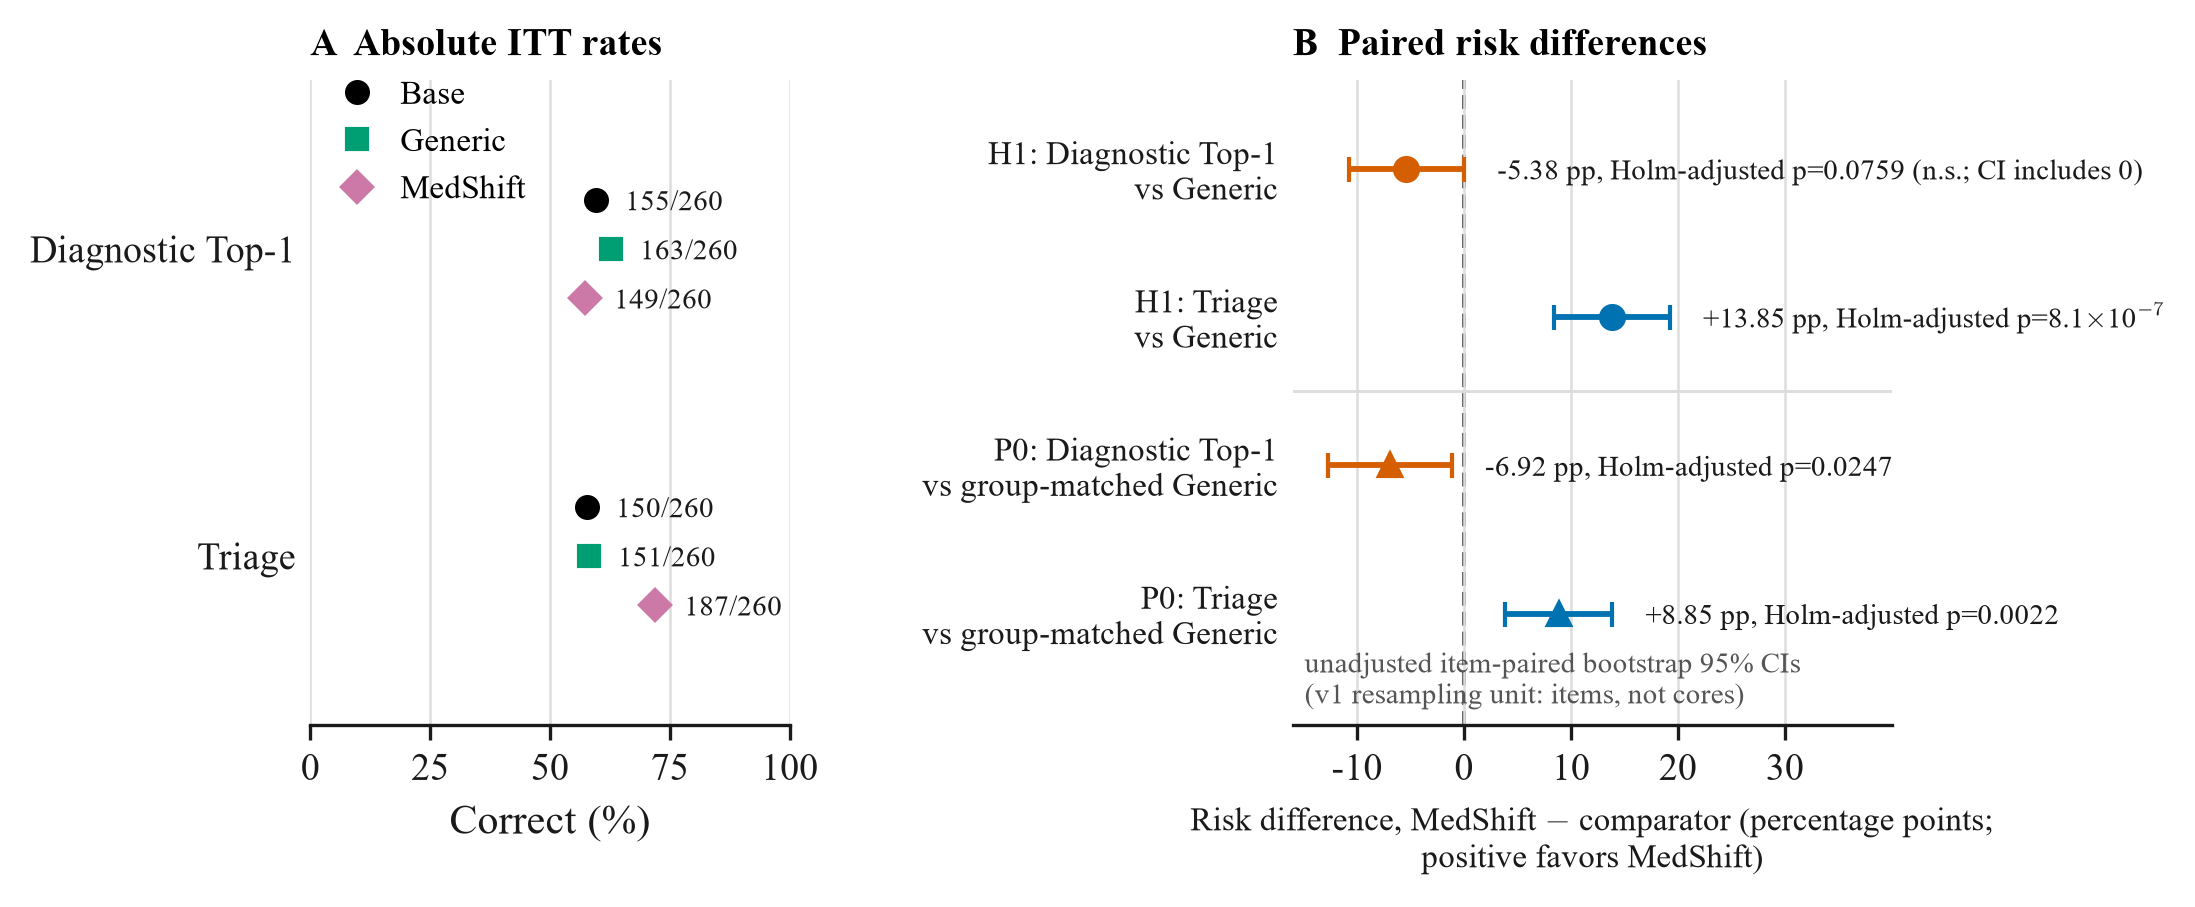
\includegraphics[width=0.92\textwidth]{figures/v1_endpoint_tradeoff.png}
\caption{\textbf{Clinical endpoint decoupling on \textsc{MedShiftBench} ($n=260$).} \textbf{Left (A):} Absolute ITT accuracy across Base, Generic LoRA, and \MedShift{} LoRA. \textbf{Right (B):} Paired risk differences (\MedShift{} $-$ Comparator) with 95\% item-paired bootstrap intervals for both the primary equal-budget H1 contrast and the prespecified P0 group-matched Generic control.}
\label{fig:tradeoff}
\end{figure*}

\subsection{Group-Matched Control (P0) and GeoShift Slice}
Because \MedShift{} contained 1,092 atomic clinical groups vs.\ 2,000 in Generic, we trained a prespecified \textbf{P0 group-matched Generic control} (1,092 records in 1,092 groups) to test whether group diversity alone explained the split. Table~\ref{tab:p0} and Figure~\ref{fig:tradeoff}B summarize P0 and the prespecified GeoShift slice:
\begin{itemize}
  \item \textbf{P0 Triage replication:} \MedShift{} still beats the group-matched control by \textbf{+8.85 pp} (187/260 vs.\ 164/260; 95\% CI $[+3.85, +13.85]$ pp; Holm $p=0.0022$), confirming the triage gain is not solely a group-count artifact. Under P0, the Top-1 gap reaches $-6.92$ pp (149/260 vs.\ 167/260; Holm $p=0.0247$), reinforcing the endpoint divergence.
  \item \textbf{GeoShift Triage slice ($n=60$):} \MedShift{} achieves \textbf{52/60 (86.7\%)} vs.\ Generic 28/60 (46.7\%) --- a \textbf{+40.00 pp} surge (95\% CI $[+26.67, +53.33]$ pp; Holm $p=8.05\times10^{-6}$), while keeping Geography control triage high (87.5\% vs.\ 85.0\%) and LanguageShift triage positive (+5.0 pp, 73.3\% vs.\ 68.3\%).
\end{itemize}

\begin{table}[t]
\centering
\caption{Prespecified P0 group-matched control ($n=260$) and supportive GeoShift triage slice ($n=60$). RD is \MedShift{} $-$ Control.}
\label{tab:p0}
\footnotesize
\setlength{\tabcolsep}{4pt}
\resizebox{\linewidth}{!}{%
\begin{tabular}{@{}lrrrrr@{}}
\toprule
Contrast & $n$ & Ctrl & \MedShift{} & RD (pp) & Holm $p$ \\
\midrule
P0 Triage (ITT) & 260 & 164 & \textbf{187} & \textbf{+8.85} & \textbf{0.0022} \\
P0 Top-1 (ITT) & 260 & 167 & 149 & $-6.92$ & 0.0247 \\
GeoShift Triage & 60 & 28 & \textbf{52} & \textbf{+40.00} & $\mathbf{8.05\times10^{-6}}$ \\
\bottomrule
\end{tabular}}
\end{table}

\section{Open-Source Reliability and Decoding Infrastructure}
Beyond the V1 benchmark results, the public \texttt{medshift} package releases four standalone modules developed to prevent silent scoring and decoding failures in clinical LLM pipelines:
\begin{enumerate}
  \item \textbf{Strict ITT statistics} (\texttt{statistics}): reproducible item-paired bootstrap, exact McNemar, Holm--Bonferroni, and effect-size reporting.
  \item \textbf{Shifted CE \& KL replay loss} (\texttt{losses}): explicit next-token shifted cross-entropy (\texttt{logits[:,:-1]} vs.\ \texttt{labels[:,1:]}) with optional KL regularization toward a frozen reference teacher to guard against off-by-one loss bugs and catastrophic forgetting.
  \item \textbf{Cached token-mask decoder} (\texttt{decoding}): deterministic finite-state schema automaton with cached vocabulary masks enforcing structured clinical sections at generation time.
  \item \textbf{Bilingual parser \& loop guards} (\texttt{guards}): canonical 8-section heading parser with diacritic-insensitive Arabic triage extraction (including plural MSA urgency forms) plus streaming periodic-token-loop and word-run detectors.
\end{enumerate}

\section{Discussion, Limitations, and Intended Use}

\paragraph{Why endpoint decoupling matters.}
Our central empirical finding is that context-shift fine-tuning can yield large, statistically decisive gains in clinical urgency recognition (+13.85 pp overall; +40.0 pp on geographic counterfactuals) without improving --- and under the group-matched control slightly lowering --- differential diagnosis Top-1 accuracy. Reporting a single composite benchmark score would mask this split. Consistent with clinical AI reporting guidelines~\cite{collins2024tripodai}, safety-critical evaluations should separate urgency escalation from diagnostic naming.

\paragraph{Limitations.}
First, \textsc{MedShiftBench} consists of author-constructed, human-reviewed clinical vignettes rather than electronic health records; improvements on constructed shifts do not prove generalization to real patient care. Second, the +40.0 pp GeoShift triage surge is compatible with both genuine epidemiological context sensitivity and geography-token heuristics~\cite{geirhos2020shortcut}. Third, Arabic evaluation covers Modern Standard Arabic only and does not capture regional spoken dialects. Fourth, V1 human adjudication recorded binary triage correctness without separate under-triage vs.\ over-triage direction labels.

\paragraph{Intended use.}
This work is an open ML research study and must not be used for clinical diagnosis, triage, or patient care. Any clinical translation would require prospective hospital validation, under-triage safety bounds, and clinician-governed escalation.

{\footnotesize
\bibliographystyle{abbrv}
\bibliography{references}
}

\end{document}
